\chapter{Method}

\section{From fMRI scans to graphs}\label{sec:fmri_to_graphs}
The data that constituted the foundation of our work is from the UK biobank \cite{ukbiobank}. This is an extensive data bank that contains genetic and biomedical information for over 500 000 subjects in the UK. Examples of types of data that is included in the biobank are subject sex, age, cognitive abilities, disease history, but also more specific information such as brain scans. 

\begin{figure}[H]
    \centering
    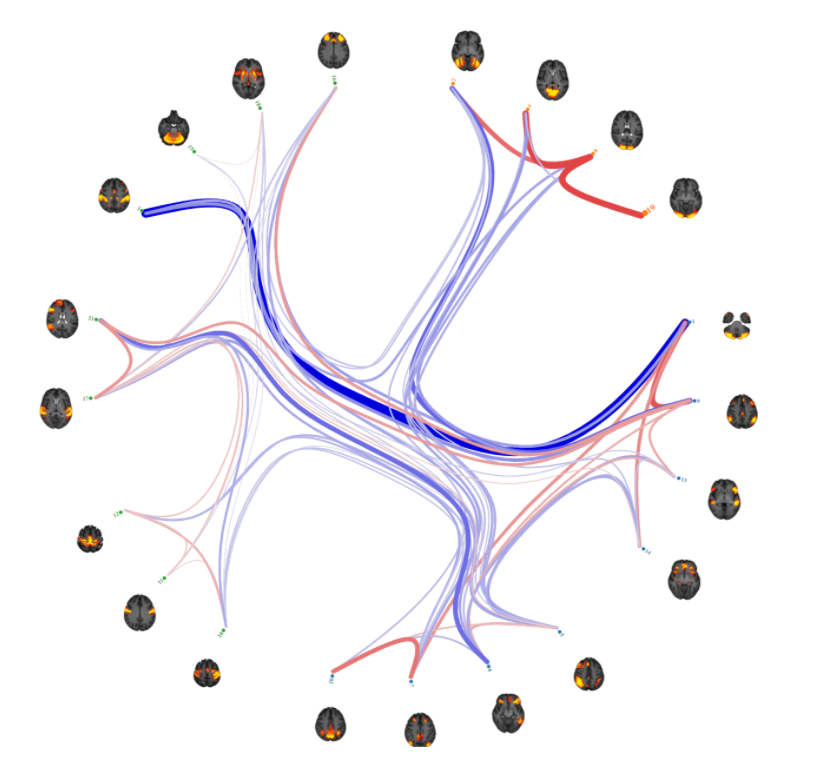
\includegraphics[width=0.7\textwidth]{chapters/images_methods/fmri_network.PNG}
    \caption{A network of functional brain network, image retrieved from UK Biobank brain imaging showcase  \cite{ukbiobank_brain_imaging}.}
    \label{fig:fmri_network}
\end{figure}

For the purpose of our project, we are specifically focusing on functional MRI brain scans, which is available for roughly 35 000 subjects varying between 45 and 80 years of age. Functional MRI (fMRI) is a technique for measuring the activation of the human brain. In a measurement, the activation of various parts of the subject brain is measured as time series. These time series can be correlated, with highly correlated regions being formed into networks. The regions that make up these network does not necessarily have to be physically close together. These networks are often associated with certain functionalities of the brain. Example of such functional networks are the vision network, responsible for processing visual stimuli, and the Defualt Mode Network (DMN), which handles memory processing and daydreaming. Multiple networks may be associated with the same functionality. In our case, groups of these networks that are related to the same functional network have been clustered together to form a 21 node \textit{network of networks}, which we represent as a graph. Each node in our fMRI-graphs thus corresponds to one functional network in the human brain (such as the DMN etc.). The weight of the edges between each of the nodes is calculated as the average correlation between the networks that make up the two nodes. A visualization of such an fMRI graph is given in figure \ref{fig:fmri_network}, in which the various nodes and the functional networks they represent form the outer circle, with the coloured lines connecting the nodes being the edges in the graph. The lines are coloured according to edge weight, with blue and red lines having negative and positive weight respectively.

\subsection{How to handle negative values - split}
Since the connections in the brain graphs was calculated from correlations the possibility of negative connection exists and in fact they occurs very often; about half of all connections are less then zero. This is a problem since the risk of dividing by zero in the normalization procedure in equation \eqref{eq:renormalization_trick} become eminent and the connections may then be uncontrollably large. There are several ways to handle this problem some alternative is to only regard positive or negative connections alone, another might be to look at the absolute value of the connections. We however decided to split the graphs negative and positive connections and create a multiplex graph \cite{}. A multiplex graph is a graph with a fixed set of nodes but with several sets of edges. One example could be when constructing a graph with cities as nodes and different means of transportation constitutes the edges. Edges representing highways and railways makes up two different graphs but they might be combined into a multiplex graph since they have the same nodes. So in our case we make two graphs one with negative connections and one with positive and combine them into a multiplex graph. From a practical point of view this was executed by creating a block diagonal adjacency matrix with the original adjacency matrix with the negative connections removed in the top left corner and the corresponding matrix with positive connections removed in the down right corner. A illustration of this can be seen in figure \ref{fig:block_diagonal_adjacency_matrix}.

\begin{figure}[H]
    \centering
    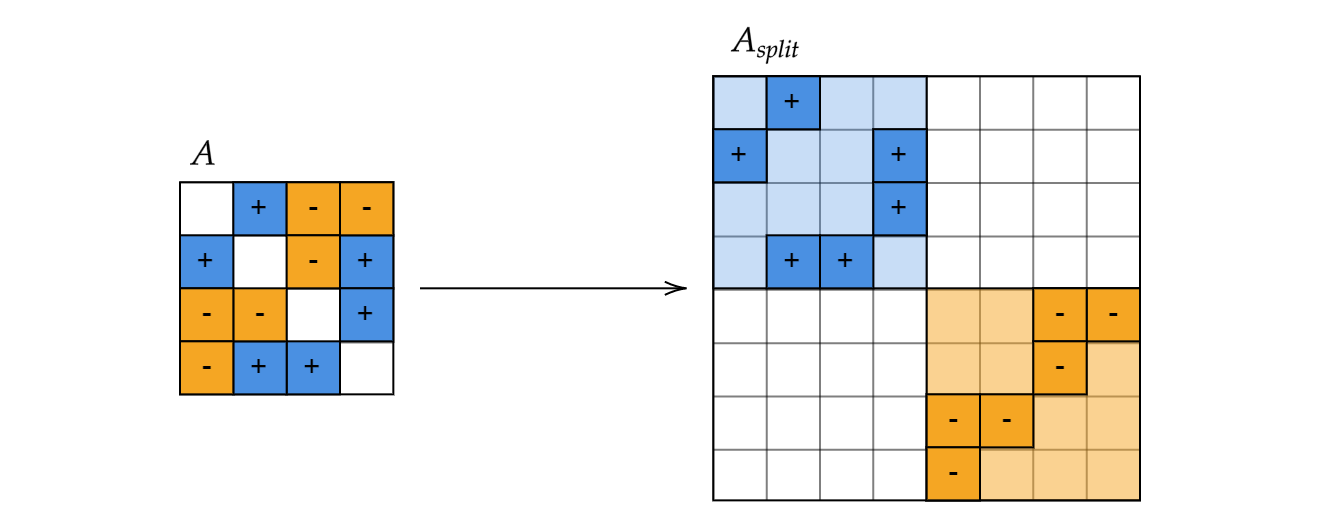
\includegraphics[width=0.9\textwidth]{chapters/images_methods/split.png}
    \caption{TEMP}
    \label{fig:block_diagonal_adjacency_matrix}
\end{figure}

Snygg figur - blockdiagonal
Stratification

\section{Graph classification -- subject-wise}
In this section all models performing graph predictions for individual subjects are introduced.

\subsection{Baseline model}
To be able to validate how well all different GCN-models performs we first need to construct some kind of baseline model to compare against. In this study the baseline model consists of a regression model where the list of all connections between all of the nodes are considered as a high dimensional data point. The reason we can consider this as a baseline model and  expect sensical results is that the obtained data over the brain graphs is ordered. Generally graphs are node ordering invariant which would be a big problem but since we can make sure the ordering of the node we can garrantie the the regression model gets connection between the same node in every data point. For schematic view off the model see figure \ref{fig:Graph_class_baseline}, where the output layer has either 2 softmax neurons for sex classification or 1 neuron without activation for age regression. 

% \begin{center}
%     \resizebox {0.9\linewidth} {!} {
%         

\tikzset{every picture/.style={line width=0.75pt}} %set default line width to 0.75pt        

\begin{tikzpicture}[x=0.75pt,y=0.75pt,yscale=-1,xscale=1]
%uncomment if require: \path (0,256); %set diagram left start at 0, and has height of 256

%Straight Lines [id:da08012385894546048] 
\draw [color={rgb, 255:red, 0; green, 0; blue, 0 }  ,draw opacity=1 ]   (45,45) -- (185,130) ;
%Straight Lines [id:da8398961471148605] 
\draw [color={rgb, 255:red, 0; green, 0; blue, 0 }  ,draw opacity=1 ]   (45,85) -- (185,130) ;
%Straight Lines [id:da8832621988467466] 
\draw [color={rgb, 255:red, 0; green, 0; blue, 0 }  ,draw opacity=1 ]   (45,125) -- (185,130) ;
%Straight Lines [id:da8658449844223002] 
\draw [color={rgb, 255:red, 0; green, 0; blue, 0 }  ,draw opacity=1 ]   (45,215) -- (185,130) ;
%Straight Lines [id:da9842325204560114] 
\draw    (220,130) -- (270,130) ;
%Straight Lines [id:da9699253287015002] 
\draw    (280,110) -- (270,130) ;
%Straight Lines [id:da3136144075299854] 
\draw    (270,130) -- (280,150) ;
%Straight Lines [id:da4214591700017929] 
\draw    (280,110) -- (318,110) ;
\draw [shift={(320,110)}, rotate = 180] [fill={rgb, 255:red, 0; green, 0; blue, 0 }  ][line width=0.08]  [draw opacity=0] (12,-3) -- (0,0) -- (12,3) -- cycle    ;
%Straight Lines [id:da7746738186045765] 
\draw    (280,150) -- (318,150) ;
\draw [shift={(320,150)}, rotate = 180] [fill={rgb, 255:red, 0; green, 0; blue, 0 }  ][line width=0.08]  [draw opacity=0] (12,-3) -- (0,0) -- (12,3) -- cycle    ;
%Shape: Axis 2D [id:dp11393948673287424] 
\draw  (430,122.25) -- (460,122.25)(433,97.47) -- (433,125) (453,117.25) -- (460,122.25) -- (453,127.25) (428,104.47) -- (433,97.47) -- (438,104.47)  ;
%Straight Lines [id:da09576460905063744] 
\draw [color={rgb, 255:red, 74; green, 144; blue, 226 }  ,draw opacity=1 ]   (430,125) -- (451.67,103.33) -- (460,95) ;
%Shape: Axis 2D [id:dp12724162882260592] 
\draw  (430,157.07) -- (460,157.07)(433,135) -- (433,159.53) (453,152.07) -- (460,157.07) -- (453,162.07) (428,142) -- (433,135) -- (438,142)  ;
%Straight Lines [id:da9285983842245029] 
\draw [color={rgb, 255:red, 208; green, 2; blue, 27 }  ,draw opacity=1 ]   (440,137) -- (440,157) ;
%Straight Lines [id:da4541122584680737] 
\draw [color={rgb, 255:red, 74; green, 144; blue, 226 }  ,draw opacity=1 ]   (450,147) -- (450,157) ;

%Shape: Circle [id:dp5473399963870353] 
\draw  [fill={rgb, 255:red, 255; green, 255; blue, 255 }  ,fill opacity=1 ] (30,45) .. controls (30,36.72) and (36.72,30) .. (45,30) .. controls (53.28,30) and (60,36.72) .. (60,45) .. controls (60,53.28) and (53.28,60) .. (45,60) .. controls (36.72,60) and (30,53.28) .. (30,45) -- cycle ;
%Shape: Circle [id:dp9366596747620268] 
\draw  [fill={rgb, 255:red, 255; green, 255; blue, 255 }  ,fill opacity=1 ] (30,215) .. controls (30,206.72) and (36.72,200) .. (45,200) .. controls (53.28,200) and (60,206.72) .. (60,215) .. controls (60,223.28) and (53.28,230) .. (45,230) .. controls (36.72,230) and (30,223.28) .. (30,215) -- cycle ;
%Shape: Circle [id:dp6370056516541169] 
\draw  [fill={rgb, 255:red, 255; green, 255; blue, 255 }  ,fill opacity=1 ] (30,125) .. controls (30,116.72) and (36.72,110) .. (45,110) .. controls (53.28,110) and (60,116.72) .. (60,125) .. controls (60,133.28) and (53.28,140) .. (45,140) .. controls (36.72,140) and (30,133.28) .. (30,125) -- cycle ;
%Shape: Circle [id:dp6076795307057334] 
\draw  [fill={rgb, 255:red, 255; green, 255; blue, 255 }  ,fill opacity=1 ] (30,85) .. controls (30,76.72) and (36.72,70) .. (45,70) .. controls (53.28,70) and (60,76.72) .. (60,85) .. controls (60,93.28) and (53.28,100) .. (45,100) .. controls (36.72,100) and (30,93.28) .. (30,85) -- cycle ;
%Shape: Circle [id:dp15718416196861162] 
\draw  [fill={rgb, 255:red, 255; green, 255; blue, 255 }  ,fill opacity=1 ] (150,130) .. controls (150,110.67) and (165.67,95) .. (185,95) .. controls (204.33,95) and (220,110.67) .. (220,130) .. controls (220,149.33) and (204.33,165) .. (185,165) .. controls (165.67,165) and (150,149.33) .. (150,130) -- cycle ;

% Text Node
\draw (37,204.4) node [anchor=north west][inner sep=0.75pt]    {$x_{n}$};
% Text Node
\draw (37,114.4) node [anchor=north west][inner sep=0.75pt]    {$x_{3}$};
% Text Node
\draw (37,74.4) node [anchor=north west][inner sep=0.75pt]    {$x_{2}$};
% Text Node
\draw (37,34.4) node [anchor=north west][inner sep=0.75pt]    {$x_{1}$};
% Text Node
\draw (84,57.4) node [anchor=north west][inner sep=0.75pt]  [font=\scriptsize,color={rgb, 255:red, 0; green, 0; blue, 0 }  ,opacity=1 ]  {${\textstyle \theta _{1}}$};
% Text Node
\draw (84,87.4) node [anchor=north west][inner sep=0.75pt]  [font=\scriptsize,color={rgb, 255:red, 0; green, 0; blue, 0 }  ,opacity=1 ]  {${\textstyle \theta _{2}}$};
% Text Node
\draw (84,114.4) node [anchor=north west][inner sep=0.75pt]  [font=\scriptsize,color={rgb, 255:red, 0; green, 0; blue, 0 }  ,opacity=1 ]  {${\textstyle \theta _{3}}$};
% Text Node
\draw (84,157.4) node [anchor=north west][inner sep=0.75pt]  [font=\scriptsize,color={rgb, 255:red, 0; green, 0; blue, 0 }  ,opacity=1 ]  {${\textstyle \theta _{n}}$};
% Text Node
\draw (151,109.4) node [anchor=north west][inner sep=0.75pt]  [font=\footnotesize]  {$\sigma \left(\sum _{i} \theta _{i} x_{i}\right)$};
% Text Node
\draw (380,130) node   [align=left] {\begin{minipage}[lt]{68pt}\setlength\topsep{0pt}
\textbf{Age}
\begin{undefined}
\textit{or}
\end{undefined}
\textbf{Male/Female}
\end{minipage}};
% Text Node
\draw (241,109.4) node [anchor=north west][inner sep=0.75pt]    {$y$};
% Text Node
\draw (34,152.4) node [anchor=north west][inner sep=0.75pt]  [font=\Large]  {$\vdots $};


\end{tikzpicture}

%     }
% \end{center}

\begin{figure}[H]
    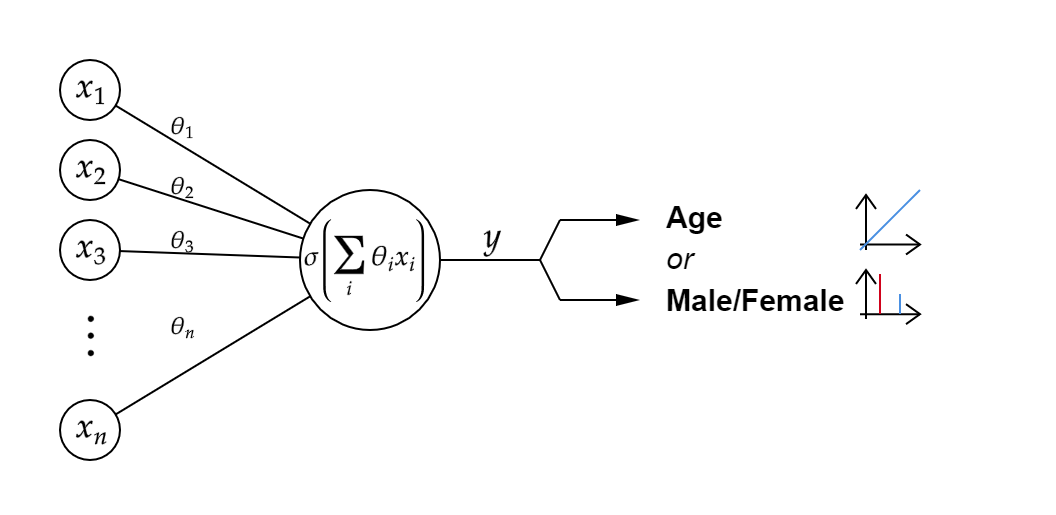
\includegraphics[width=0.9\textwidth]{chapters/images_methods/ffnn.png}
    \caption{TEMP}
    \label{fig:Graph_class_baseline}
\end{figure}

\subsection{GCN base}
The first model, which is refereed to as GCNBase, consists of 3 consecutive graph convolutional layers, with propagation rule seen in \eqref{eq:propagation_rule}, and a fully connected output layer. The GCN layers will always have the rectified linear unit (RELU) as activation function and ten output features, unless otherwise specified. The input to the fully connected output layer consisted of all the activation's after all three GCN layers, i.e. the activation for all feature maps in all layers. As described in the section \ref{sec:gcn} the activation of layers $i$ will contain information about the $i$-order neighbourhood of each node. The inclusion of activation's after each layer thus aims to utilize information of how each node is embedded in a larger and larger neighbourhood, which could be important for the prediction.

%The activation of each layer will contain information of a larger and larger local neighbourhood of nodes in the graph. Therefor after the GCN layers we concatenate all activation's in all layers and feed them to a regular dense layer with either two softmax neurons or one without activation as output just as the baseline model.

% \begin{center}
%     \resizebox {0.9\linewidth} {!} {
%         

\tikzset{every picture/.style={line width=0.75pt}} %set default line width to 0.75pt        

\begin{tikzpicture}[x=0.75pt,y=0.75pt,yscale=-1,xscale=1]
%uncomment if require: \path (0,268); %set diagram left start at 0, and has height of 268

%Rounded Rect [id:dp1454512597044859] 
\draw  [fill={rgb, 255:red, 255; green, 255; blue, 255 }  ,fill opacity=1 ] (150,48) .. controls (150,38.06) and (158.06,30) .. (168,30) -- (222,30) .. controls (231.94,30) and (240,38.06) .. (240,48) -- (240,222) .. controls (240,231.94) and (231.94,240) .. (222,240) -- (168,240) .. controls (158.06,240) and (150,231.94) .. (150,222) -- cycle ;
%Straight Lines [id:da44371133423221676] 
\draw [color={rgb, 255:red, 155; green, 155; blue, 155 }  ,draw opacity=1 ][line width=1.5]    (169.29,109.19) -- (177.86,134.65) ;
%Straight Lines [id:da3398362409006068] 
\draw [color={rgb, 255:red, 155; green, 155; blue, 155 }  ,draw opacity=1 ][line width=1.5]    (169.29,109.19) -- (195,96.46) ;
%Shape: Ellipse [id:dp7222477940626566] 
\draw  [color={rgb, 255:red, 245; green, 166; blue, 35 }  ,draw opacity=1 ][fill={rgb, 255:red, 245; green, 166; blue, 35 }  ,fill opacity=1 ] (165,109.19) .. controls (165,106.85) and (166.92,104.95) .. (169.29,104.95) .. controls (171.65,104.95) and (173.57,106.85) .. (173.57,109.19) .. controls (173.57,111.53) and (171.65,113.43) .. (169.29,113.43) .. controls (166.92,113.43) and (165,111.53) .. (165,109.19) -- cycle ;
%Straight Lines [id:da7434143201874741] 
\draw [color={rgb, 255:red, 155; green, 155; blue, 155 }  ,draw opacity=1 ][line width=1.5]    (199.29,63.23) -- (195,42.02) ;
%Straight Lines [id:da17541088644592207] 
\draw [color={rgb, 255:red, 155; green, 155; blue, 155 }  ,draw opacity=0.4 ][line width=1.5]    (177.86,80.2) -- (195,42.02) ;
%Straight Lines [id:da49554490131335505] 
\draw [color={rgb, 255:red, 155; green, 155; blue, 155 }  ,draw opacity=0.4 ][line width=1.5]    (169.29,54.75) -- (177.86,80.2) ;
%Straight Lines [id:da7823220018723711] 
\draw [color={rgb, 255:red, 155; green, 155; blue, 155 }  ,draw opacity=1 ][line width=1.5]    (199.29,63.23) -- (220.71,50.51) ;
%Straight Lines [id:da4144720186472177] 
\draw [color={rgb, 255:red, 155; green, 155; blue, 155 }  ,draw opacity=0.4 ][fill={rgb, 255:red, 0; green, 0; blue, 0 }  ,fill opacity=0.5 ][line width=1.5]    (169.29,54.75) -- (195,42.02) ;
%Straight Lines [id:da4512038117618906] 
\draw [color={rgb, 255:red, 155; green, 155; blue, 155 }  ,draw opacity=1 ][line width=1.5]    (199.29,63.23) -- (177.86,80.2) ;
%Straight Lines [id:da6717586155874848] 
\draw [color={rgb, 255:red, 155; green, 155; blue, 155 }  ,draw opacity=1 ][line width=1.5]    (199.29,63.23) -- (216.43,75.96) ;
%Shape: Ellipse [id:dp8214542913209517] 
\draw  [color={rgb, 255:red, 167; green, 207; blue, 255 }  ,draw opacity=1 ][fill={rgb, 255:red, 167; green, 207; blue, 255 }  ,fill opacity=1 ] (165,54.75) .. controls (165,52.4) and (166.92,50.51) .. (169.29,50.51) .. controls (171.65,50.51) and (173.57,52.4) .. (173.57,54.75) .. controls (173.57,57.09) and (171.65,58.99) .. (169.29,58.99) .. controls (166.92,58.99) and (165,57.09) .. (165,54.75) -- cycle ;
%Shape: Ellipse [id:dp47038889017471486] 
\draw  [color={rgb, 255:red, 74; green, 144; blue, 226 }  ,draw opacity=1 ][fill={rgb, 255:red, 74; green, 144; blue, 226 }  ,fill opacity=1 ] (173.57,80.2) .. controls (173.57,77.86) and (175.49,75.96) .. (177.86,75.96) .. controls (180.22,75.96) and (182.14,77.86) .. (182.14,80.2) .. controls (182.14,82.55) and (180.22,84.44) .. (177.86,84.44) .. controls (175.49,84.44) and (173.57,82.55) .. (173.57,80.2) -- cycle ;
%Shape: Ellipse [id:dp10306056601214997] 
\draw  [color={rgb, 255:red, 245; green, 166; blue, 35 }  ,draw opacity=1 ][fill={rgb, 255:red, 245; green, 166; blue, 35 }  ,fill opacity=1 ] (195,63.23) .. controls (195,60.89) and (196.92,58.99) .. (199.29,58.99) .. controls (201.65,58.99) and (203.57,60.89) .. (203.57,63.23) .. controls (203.57,65.58) and (201.65,67.47) .. (199.29,67.47) .. controls (196.92,67.47) and (195,65.58) .. (195,63.23) -- cycle ;
%Shape: Ellipse [id:dp3356200716848863] 
\draw  [color={rgb, 255:red, 74; green, 144; blue, 226 }  ,draw opacity=1 ][fill={rgb, 255:red, 74; green, 144; blue, 226 }  ,fill opacity=1 ] (212.14,75.96) .. controls (212.14,73.62) and (214.06,71.72) .. (216.43,71.72) .. controls (218.8,71.72) and (220.71,73.62) .. (220.71,75.96) .. controls (220.71,78.3) and (218.8,80.2) .. (216.43,80.2) .. controls (214.06,80.2) and (212.14,78.3) .. (212.14,75.96) -- cycle ;
%Shape: Ellipse [id:dp9107615531803757] 
\draw  [color={rgb, 255:red, 74; green, 144; blue, 226 }  ,draw opacity=1 ][fill={rgb, 255:red, 74; green, 144; blue, 226 }  ,fill opacity=1 ] (190.71,42.02) .. controls (190.71,39.68) and (192.63,37.78) .. (195,37.78) .. controls (197.37,37.78) and (199.29,39.68) .. (199.29,42.02) .. controls (199.29,44.36) and (197.37,46.26) .. (195,46.26) .. controls (192.63,46.26) and (190.71,44.36) .. (190.71,42.02) -- cycle ;
%Shape: Ellipse [id:dp686194905732459] 
\draw  [color={rgb, 255:red, 74; green, 144; blue, 226 }  ,draw opacity=1 ][fill={rgb, 255:red, 74; green, 144; blue, 226 }  ,fill opacity=1 ] (216.43,50.51) .. controls (216.43,48.16) and (218.35,46.26) .. (220.71,46.26) .. controls (223.08,46.26) and (225,48.16) .. (225,50.51) .. controls (225,52.85) and (223.08,54.75) .. (220.71,54.75) .. controls (218.35,54.75) and (216.43,52.85) .. (216.43,50.51) -- cycle ;
%Straight Lines [id:da4462253100757778] 
\draw [color={rgb, 255:red, 155; green, 155; blue, 155 }  ,draw opacity=1 ][line width=1.5]    (177.86,227.98) -- (195,189.8) ;
%Straight Lines [id:da33046752635028676] 
\draw [color={rgb, 255:red, 155; green, 155; blue, 155 }  ,draw opacity=1 ][line width=1.5]    (169.29,202.53) -- (177.86,227.98) ;
%Straight Lines [id:da45388559372006365] 
\draw [color={rgb, 255:red, 155; green, 155; blue, 155 }  ,draw opacity=1 ][line width=1.5]    (199.29,211.01) -- (177.86,227.98) ;
%Shape: Ellipse [id:dp12334564292514116] 
\draw  [color={rgb, 255:red, 245; green, 166; blue, 35 }  ,draw opacity=1 ][fill={rgb, 255:red, 245; green, 166; blue, 35 }  ,fill opacity=1 ] (173.57,227.98) .. controls (173.57,225.64) and (175.49,223.74) .. (177.86,223.74) .. controls (180.22,223.74) and (182.14,225.64) .. (182.14,227.98) .. controls (182.14,230.32) and (180.22,232.22) .. (177.86,232.22) .. controls (175.49,232.22) and (173.57,230.32) .. (173.57,227.98) -- cycle ;
%Straight Lines [id:da5879944549609841] 
\draw [color={rgb, 255:red, 155; green, 155; blue, 155 }  ,draw opacity=0.4 ][fill={rgb, 255:red, 0; green, 0; blue, 0 }  ,fill opacity=0.5 ][line width=1.5]    (195,96.46) -- (177.86,134.65) ;
%Straight Lines [id:da10478801456064013] 
\draw [color={rgb, 255:red, 155; green, 155; blue, 155 }  ,draw opacity=0.4 ][fill={rgb, 255:red, 0; green, 0; blue, 0 }  ,fill opacity=0.5 ][line width=1.5]    (195,96.46) -- (199.29,117.68) ;
%Straight Lines [id:da5465003287874521] 
\draw [color={rgb, 255:red, 155; green, 155; blue, 155 }  ,draw opacity=0.4 ][fill={rgb, 255:red, 0; green, 0; blue, 0 }  ,fill opacity=0.5 ][line width=1.5]    (177.86,134.65) -- (199.29,117.68) ;
%Straight Lines [id:da029197166814233233] 
\draw [color={rgb, 255:red, 155; green, 155; blue, 155 }  ,draw opacity=0.4 ][fill={rgb, 255:red, 0; green, 0; blue, 0 }  ,fill opacity=0.5 ][line width=1.5]    (199.29,117.68) -- (220.71,104.95) ;
%Straight Lines [id:da7886430348639939] 
\draw [color={rgb, 255:red, 155; green, 155; blue, 155 }  ,draw opacity=0.4 ][fill={rgb, 255:red, 0; green, 0; blue, 0 }  ,fill opacity=0.5 ][line width=1.5]    (199.29,117.68) -- (216.43,130.4) ;
%Straight Lines [id:da48838206548505325] 
\draw [color={rgb, 255:red, 155; green, 155; blue, 155 }  ,draw opacity=0.4 ][fill={rgb, 255:red, 0; green, 0; blue, 0 }  ,fill opacity=0.5 ][line width=1.5]    (195,189.8) -- (169.29,202.53) ;
%Straight Lines [id:da6023020962352053] 
\draw [color={rgb, 255:red, 155; green, 155; blue, 155 }  ,draw opacity=0.4 ][fill={rgb, 255:red, 0; green, 0; blue, 0 }  ,fill opacity=0.5 ][line width=1.5]    (195,189.8) -- (199.29,211.01) ;
%Straight Lines [id:da9783904688690421] 
\draw [color={rgb, 255:red, 155; green, 155; blue, 155 }  ,draw opacity=0.4 ][fill={rgb, 255:red, 0; green, 0; blue, 0 }  ,fill opacity=0.5 ][line width=1.5]    (220.71,198.28) -- (199.29,211.01) ;
%Shape: Ellipse [id:dp3754045964979047] 
\draw  [color={rgb, 255:red, 74; green, 144; blue, 226 }  ,draw opacity=1 ][fill={rgb, 255:red, 74; green, 144; blue, 226 }  ,fill opacity=1 ] (190.71,189.8) .. controls (190.71,187.45) and (192.63,185.56) .. (195,185.56) .. controls (197.37,185.56) and (199.29,187.45) .. (199.29,189.8) .. controls (199.29,192.14) and (197.37,194.04) .. (195,194.04) .. controls (192.63,194.04) and (190.71,192.14) .. (190.71,189.8) -- cycle ;
%Shape: Ellipse [id:dp64113309900183] 
\draw  [color={rgb, 255:red, 167; green, 207; blue, 255 }  ,draw opacity=1 ][fill={rgb, 255:red, 167; green, 207; blue, 255 }  ,fill opacity=1 ] (216.43,198.28) .. controls (216.43,195.94) and (218.35,194.04) .. (220.71,194.04) .. controls (223.08,194.04) and (225,195.94) .. (225,198.28) .. controls (225,200.63) and (223.08,202.53) .. (220.71,202.53) .. controls (218.35,202.53) and (216.43,200.63) .. (216.43,198.28) -- cycle ;
%Shape: Ellipse [id:dp691449696768264] 
\draw  [color={rgb, 255:red, 74; green, 144; blue, 226 }  ,draw opacity=1 ][fill={rgb, 255:red, 74; green, 144; blue, 226 }  ,fill opacity=1 ] (165,202.53) .. controls (165,200.18) and (166.92,198.28) .. (169.29,198.28) .. controls (171.65,198.28) and (173.57,200.18) .. (173.57,202.53) .. controls (173.57,204.87) and (171.65,206.77) .. (169.29,206.77) .. controls (166.92,206.77) and (165,204.87) .. (165,202.53) -- cycle ;
%Straight Lines [id:da03064657141642635] 
\draw [color={rgb, 255:red, 155; green, 155; blue, 155 }  ,draw opacity=0.4 ][fill={rgb, 255:red, 0; green, 0; blue, 0 }  ,fill opacity=0.5 ][line width=1.5]    (216.43,223.74) -- (199.29,211.01) ;
%Shape: Ellipse [id:dp07058389708117052] 
\draw  [color={rgb, 255:red, 74; green, 144; blue, 226 }  ,draw opacity=1 ][fill={rgb, 255:red, 74; green, 144; blue, 226 }  ,fill opacity=1 ] (195,211.01) .. controls (195,208.67) and (196.92,206.77) .. (199.29,206.77) .. controls (201.65,206.77) and (203.57,208.67) .. (203.57,211.01) .. controls (203.57,213.35) and (201.65,215.25) .. (199.29,215.25) .. controls (196.92,215.25) and (195,213.35) .. (195,211.01) -- cycle ;
%Shape: Ellipse [id:dp697421628639054] 
\draw  [color={rgb, 255:red, 167; green, 207; blue, 255 }  ,draw opacity=1 ][fill={rgb, 255:red, 167; green, 207; blue, 255 }  ,fill opacity=1 ] (212.14,223.74) .. controls (212.14,221.39) and (214.06,219.49) .. (216.43,219.49) .. controls (218.8,219.49) and (220.71,221.39) .. (220.71,223.74) .. controls (220.71,226.08) and (218.8,227.98) .. (216.43,227.98) .. controls (214.06,227.98) and (212.14,226.08) .. (212.14,223.74) -- cycle ;
%Shape: Ellipse [id:dp8717393277655574] 
\draw  [color={rgb, 255:red, 167; green, 207; blue, 255 }  ,draw opacity=1 ][fill={rgb, 255:red, 167; green, 207; blue, 255 }  ,fill opacity=1 ] (195,117.68) .. controls (195,115.33) and (196.92,113.43) .. (199.29,113.43) .. controls (201.65,113.43) and (203.57,115.33) .. (203.57,117.68) .. controls (203.57,120.02) and (201.65,121.92) .. (199.29,121.92) .. controls (196.92,121.92) and (195,120.02) .. (195,117.68) -- cycle ;
%Shape: Ellipse [id:dp770793755049425] 
\draw  [color={rgb, 255:red, 167; green, 207; blue, 255 }  ,draw opacity=1 ][fill={rgb, 255:red, 167; green, 207; blue, 255 }  ,fill opacity=1 ] (212.14,130.4) .. controls (212.14,128.06) and (214.06,126.16) .. (216.43,126.16) .. controls (218.8,126.16) and (220.71,128.06) .. (220.71,130.4) .. controls (220.71,132.75) and (218.8,134.65) .. (216.43,134.65) .. controls (214.06,134.65) and (212.14,132.75) .. (212.14,130.4) -- cycle ;
%Shape: Ellipse [id:dp6425563981873512] 
\draw  [color={rgb, 255:red, 167; green, 207; blue, 255 }  ,draw opacity=1 ][fill={rgb, 255:red, 167; green, 207; blue, 255 }  ,fill opacity=1 ] (216.43,104.95) .. controls (216.43,102.61) and (218.35,100.71) .. (220.71,100.71) .. controls (223.08,100.71) and (225,102.61) .. (225,104.95) .. controls (225,107.29) and (223.08,109.19) .. (220.71,109.19) .. controls (218.35,109.19) and (216.43,107.29) .. (216.43,104.95) -- cycle ;
%Shape: Ellipse [id:dp6740261081738981] 
\draw  [color={rgb, 255:red, 74; green, 144; blue, 226 }  ,draw opacity=1 ][fill={rgb, 255:red, 74; green, 144; blue, 226 }  ,fill opacity=1 ] (190.71,96.46) .. controls (190.71,94.12) and (192.63,92.22) .. (195,92.22) .. controls (197.37,92.22) and (199.29,94.12) .. (199.29,96.46) .. controls (199.29,98.81) and (197.37,100.71) .. (195,100.71) .. controls (192.63,100.71) and (190.71,98.81) .. (190.71,96.46) -- cycle ;
%Shape: Ellipse [id:dp04602563531483872] 
\draw  [color={rgb, 255:red, 74; green, 144; blue, 226 }  ,draw opacity=1 ][fill={rgb, 255:red, 74; green, 144; blue, 226 }  ,fill opacity=1 ] (173.57,134.65) .. controls (173.57,132.3) and (175.49,130.4) .. (177.86,130.4) .. controls (180.22,130.4) and (182.14,132.3) .. (182.14,134.65) .. controls (182.14,136.99) and (180.22,138.89) .. (177.86,138.89) .. controls (175.49,138.89) and (173.57,136.99) .. (173.57,134.65) -- cycle ;
%Shape: Ellipse [id:dp7012237407172539] 
\draw  [fill={rgb, 255:red, 0; green, 0; blue, 0 }  ,fill opacity=1 ] (193.5,159.89) .. controls (193.5,158.6) and (194.51,157.56) .. (195.75,157.56) .. controls (196.99,157.56) and (198,158.6) .. (198,159.89) .. controls (198,161.18) and (196.99,162.22) .. (195.75,162.22) .. controls (194.51,162.22) and (193.5,161.18) .. (193.5,159.89) -- cycle ;
%Shape: Ellipse [id:dp3114230595274974] 
\draw  [fill={rgb, 255:red, 0; green, 0; blue, 0 }  ,fill opacity=1 ] (193.5,150.56) .. controls (193.5,149.27) and (194.51,148.22) .. (195.75,148.22) .. controls (196.99,148.22) and (198,149.27) .. (198,150.56) .. controls (198,151.84) and (196.99,152.89) .. (195.75,152.89) .. controls (194.51,152.89) and (193.5,151.84) .. (193.5,150.56) -- cycle ;
%Shape: Ellipse [id:dp37386234270345065] 
\draw  [fill={rgb, 255:red, 0; green, 0; blue, 0 }  ,fill opacity=1 ] (193.5,169.22) .. controls (193.5,167.93) and (194.51,166.89) .. (195.75,166.89) .. controls (196.99,166.89) and (198,167.93) .. (198,169.22) .. controls (198,170.51) and (196.99,171.56) .. (195.75,171.56) .. controls (194.51,171.56) and (193.5,170.51) .. (193.5,169.22) -- cycle ;

%Rounded Rect [id:dp9087802921841164] 
\draw   (260,128) .. controls (260,123.58) and (263.58,120) .. (268,120) -- (302,120) .. controls (306.42,120) and (310,123.58) .. (310,128) -- (310,152) .. controls (310,156.42) and (306.42,160) .. (302,160) -- (268,160) .. controls (263.58,160) and (260,156.42) .. (260,152) -- cycle ;
%Straight Lines [id:da04447467340422939] 
\draw    (310,140) -- (330,140) ;
%Straight Lines [id:da5334327028246098] 
\draw [color={rgb, 255:red, 155; green, 155; blue, 155 }  ,draw opacity=1 ][line width=1.5]    (65.01,142.73) -- (59.17,115.45) ;
%Straight Lines [id:da4099968368068212] 
\draw [color={rgb, 255:red, 155; green, 155; blue, 155 }  ,draw opacity=1 ][line width=1.5]    (35.85,164.55) -- (59.17,115.45) ;
%Straight Lines [id:da8075613001249213] 
\draw [color={rgb, 255:red, 155; green, 155; blue, 155 }  ,draw opacity=1 ][line width=1.5]    (24.18,131.82) -- (35.85,164.55) ;
%Straight Lines [id:da7949764047700321] 
\draw [color={rgb, 255:red, 155; green, 155; blue, 155 }  ,draw opacity=1 ][line width=1.5]    (65.01,142.73) -- (94.17,126.36) ;
%Straight Lines [id:da4886477553077586] 
\draw [color={rgb, 255:red, 155; green, 155; blue, 155 }  ,draw opacity=1 ][line width=1.5]    (24.18,131.82) -- (59.17,115.45) ;
%Straight Lines [id:da4437033864911011] 
\draw [color={rgb, 255:red, 155; green, 155; blue, 155 }  ,draw opacity=1 ][line width=1.5]    (65.01,142.73) -- (35.85,164.55) ;
%Straight Lines [id:da6182912079509322] 
\draw [color={rgb, 255:red, 155; green, 155; blue, 155 }  ,draw opacity=1 ][line width=1.5]    (65.01,142.73) -- (88.34,159.09) ;
%Shape: Ellipse [id:dp11646472758372184] 
\draw  [color={rgb, 255:red, 74; green, 144; blue, 226 }  ,draw opacity=1 ][fill={rgb, 255:red, 74; green, 144; blue, 226 }  ,fill opacity=1 ] (18.35,131.82) .. controls (18.35,128.81) and (20.96,126.36) .. (24.18,126.36) .. controls (27.4,126.36) and (30.01,128.81) .. (30.01,131.82) .. controls (30.01,134.83) and (27.4,137.27) .. (24.18,137.27) .. controls (20.96,137.27) and (18.35,134.83) .. (18.35,131.82) -- cycle ;
%Shape: Ellipse [id:dp0497507523482601] 
\draw  [color={rgb, 255:red, 74; green, 144; blue, 226 }  ,draw opacity=1 ][fill={rgb, 255:red, 74; green, 144; blue, 226 }  ,fill opacity=1 ] (30.01,164.55) .. controls (30.01,161.53) and (32.63,159.09) .. (35.85,159.09) .. controls (39.07,159.09) and (41.68,161.53) .. (41.68,164.55) .. controls (41.68,167.56) and (39.07,170) .. (35.85,170) .. controls (32.63,170) and (30.01,167.56) .. (30.01,164.55) -- cycle ;
%Shape: Ellipse [id:dp923504470392968] 
\draw  [color={rgb, 255:red, 74; green, 144; blue, 226 }  ,draw opacity=1 ][fill={rgb, 255:red, 74; green, 144; blue, 226 }  ,fill opacity=1 ] (59.17,142.73) .. controls (59.17,139.71) and (61.79,137.27) .. (65.01,137.27) .. controls (68.23,137.27) and (70.84,139.71) .. (70.84,142.73) .. controls (70.84,145.74) and (68.23,148.18) .. (65.01,148.18) .. controls (61.79,148.18) and (59.17,145.74) .. (59.17,142.73) -- cycle ;
%Shape: Ellipse [id:dp44760031358442776] 
\draw  [color={rgb, 255:red, 74; green, 144; blue, 226 }  ,draw opacity=1 ][fill={rgb, 255:red, 74; green, 144; blue, 226 }  ,fill opacity=1 ] (82.5,159.09) .. controls (82.5,156.08) and (85.11,153.64) .. (88.34,153.64) .. controls (91.56,153.64) and (94.17,156.08) .. (94.17,159.09) .. controls (94.17,162.1) and (91.56,164.55) .. (88.34,164.55) .. controls (85.11,164.55) and (82.5,162.1) .. (82.5,159.09) -- cycle ;
%Shape: Ellipse [id:dp0773933591251863] 
\draw  [color={rgb, 255:red, 74; green, 144; blue, 226 }  ,draw opacity=1 ][fill={rgb, 255:red, 74; green, 144; blue, 226 }  ,fill opacity=1 ] (53.34,115.45) .. controls (53.34,112.44) and (55.95,110) .. (59.17,110) .. controls (62.4,110) and (65.01,112.44) .. (65.01,115.45) .. controls (65.01,118.47) and (62.4,120.91) .. (59.17,120.91) .. controls (55.95,120.91) and (53.34,118.47) .. (53.34,115.45) -- cycle ;
%Shape: Ellipse [id:dp4981680059611522] 
\draw  [color={rgb, 255:red, 74; green, 144; blue, 226 }  ,draw opacity=1 ][fill={rgb, 255:red, 74; green, 144; blue, 226 }  ,fill opacity=1 ] (88.34,126.36) .. controls (88.34,123.35) and (90.95,120.91) .. (94.17,120.91) .. controls (97.39,120.91) and (100,123.35) .. (100,126.36) .. controls (100,129.38) and (97.39,131.82) .. (94.17,131.82) .. controls (90.95,131.82) and (88.34,129.38) .. (88.34,126.36) -- cycle ;

%Rounded Rect [id:dp855215770961127] 
\draw   (10,116) .. controls (10,107.16) and (17.16,100) .. (26,100) -- (94,100) .. controls (102.84,100) and (110,107.16) .. (110,116) -- (110,164) .. controls (110,172.84) and (102.84,180) .. (94,180) -- (26,180) .. controls (17.16,180) and (10,172.84) .. (10,164) -- cycle ;
%Straight Lines [id:da865822603980609] 
\draw    (110,140) -- (150,140) ;
%Straight Lines [id:da4781293941355824] 
\draw    (420,140) -- (470,140) ;
%Straight Lines [id:da9997190507560019] 
\draw    (480,120) -- (470,140) ;
%Straight Lines [id:da9897698727052839] 
\draw    (470,140) -- (480,160) ;
%Straight Lines [id:da5250020646100277] 
\draw    (480,120) -- (518,120) ;
\draw [shift={(520,120)}, rotate = 180] [fill={rgb, 255:red, 0; green, 0; blue, 0 }  ][line width=0.08]  [draw opacity=0] (12,-3) -- (0,0) -- (12,3) -- cycle    ;
%Straight Lines [id:da8007130287528326] 
\draw    (480,160) -- (518,160) ;
\draw [shift={(520,160)}, rotate = 180] [fill={rgb, 255:red, 0; green, 0; blue, 0 }  ][line width=0.08]  [draw opacity=0] (12,-3) -- (0,0) -- (12,3) -- cycle    ;
%Shape: Axis 2D [id:dp12898164037662085] 
\draw  (630,132.25) -- (660,132.25)(633,107.47) -- (633,135) (653,127.25) -- (660,132.25) -- (653,137.25) (628,114.47) -- (633,107.47) -- (638,114.47)  ;
%Straight Lines [id:da8546091575274994] 
\draw [color={rgb, 255:red, 74; green, 144; blue, 226 }  ,draw opacity=1 ]   (630,135) -- (651.67,113.33) -- (660,105) ;
%Shape: Axis 2D [id:dp3159900508610336] 
\draw  (630,167.07) -- (660,167.07)(633,145) -- (633,169.53) (653,162.07) -- (660,167.07) -- (653,172.07) (628,152) -- (633,145) -- (638,152)  ;
%Straight Lines [id:da2214390871002745] 
\draw [color={rgb, 255:red, 208; green, 2; blue, 27 }  ,draw opacity=1 ]   (640,147) -- (640,167) ;
%Straight Lines [id:da5235485948286522] 
\draw [color={rgb, 255:red, 74; green, 144; blue, 226 }  ,draw opacity=1 ]   (650,157) -- (650,167) ;

%Straight Lines [id:da0011855880200477564] 
\draw    (240,140) -- (260,140) ;
%Rounded Rect [id:dp3640479469957574] 
\draw  [fill={rgb, 255:red, 255; green, 255; blue, 255 }  ,fill opacity=1 ] (330,48) .. controls (330,38.06) and (338.06,30) .. (348,30) -- (402,30) .. controls (411.94,30) and (420,38.06) .. (420,48) -- (420,222) .. controls (420,231.94) and (411.94,240) .. (402,240) -- (348,240) .. controls (338.06,240) and (330,231.94) .. (330,222) -- cycle ;
%Straight Lines [id:da36833369698003215] 
\draw [color={rgb, 255:red, 155; green, 155; blue, 155 }  ,draw opacity=1 ][line width=1.5]    (349.29,109.19) -- (357.86,134.65) ;
%Straight Lines [id:da7140367877186562] 
\draw [color={rgb, 255:red, 155; green, 155; blue, 155 }  ,draw opacity=1 ][line width=1.5]    (349.29,109.19) -- (375,96.46) ;
%Shape: Ellipse [id:dp30211957071106843] 
\draw  [color={rgb, 255:red, 245; green, 166; blue, 35 }  ,draw opacity=1 ][fill={rgb, 255:red, 245; green, 166; blue, 35 }  ,fill opacity=1 ] (345,109.19) .. controls (345,106.85) and (346.92,104.95) .. (349.29,104.95) .. controls (351.65,104.95) and (353.57,106.85) .. (353.57,109.19) .. controls (353.57,111.53) and (351.65,113.43) .. (349.29,113.43) .. controls (346.92,113.43) and (345,111.53) .. (345,109.19) -- cycle ;
%Straight Lines [id:da17408965111455865] 
\draw [color={rgb, 255:red, 155; green, 155; blue, 155 }  ,draw opacity=1 ][line width=1.5]    (379.29,63.23) -- (375,42.02) ;
%Straight Lines [id:da08473532854907884] 
\draw [color={rgb, 255:red, 155; green, 155; blue, 155 }  ,draw opacity=0.4 ][line width=1.5]    (357.86,80.2) -- (375,42.02) ;
%Straight Lines [id:da5880812032491216] 
\draw [color={rgb, 255:red, 155; green, 155; blue, 155 }  ,draw opacity=0.4 ][line width=1.5]    (349.29,54.75) -- (357.86,80.2) ;
%Straight Lines [id:da9621297667966422] 
\draw [color={rgb, 255:red, 155; green, 155; blue, 155 }  ,draw opacity=1 ][line width=1.5]    (379.29,63.23) -- (400.71,50.51) ;
%Straight Lines [id:da6752975937599959] 
\draw [color={rgb, 255:red, 155; green, 155; blue, 155 }  ,draw opacity=0.4 ][fill={rgb, 255:red, 0; green, 0; blue, 0 }  ,fill opacity=0.5 ][line width=1.5]    (349.29,54.75) -- (375,42.02) ;
%Straight Lines [id:da09574905139243506] 
\draw [color={rgb, 255:red, 155; green, 155; blue, 155 }  ,draw opacity=1 ][line width=1.5]    (379.29,63.23) -- (357.86,80.2) ;
%Straight Lines [id:da010518874424237268] 
\draw [color={rgb, 255:red, 155; green, 155; blue, 155 }  ,draw opacity=1 ][line width=1.5]    (379.29,63.23) -- (396.43,75.96) ;
%Shape: Ellipse [id:dp8663719631601869] 
\draw  [color={rgb, 255:red, 167; green, 207; blue, 255 }  ,draw opacity=1 ][fill={rgb, 255:red, 167; green, 207; blue, 255 }  ,fill opacity=1 ] (345,54.75) .. controls (345,52.4) and (346.92,50.51) .. (349.29,50.51) .. controls (351.65,50.51) and (353.57,52.4) .. (353.57,54.75) .. controls (353.57,57.09) and (351.65,58.99) .. (349.29,58.99) .. controls (346.92,58.99) and (345,57.09) .. (345,54.75) -- cycle ;
%Shape: Ellipse [id:dp18827652152933672] 
\draw  [color={rgb, 255:red, 74; green, 144; blue, 226 }  ,draw opacity=1 ][fill={rgb, 255:red, 74; green, 144; blue, 226 }  ,fill opacity=1 ] (353.57,80.2) .. controls (353.57,77.86) and (355.49,75.96) .. (357.86,75.96) .. controls (360.22,75.96) and (362.14,77.86) .. (362.14,80.2) .. controls (362.14,82.55) and (360.22,84.44) .. (357.86,84.44) .. controls (355.49,84.44) and (353.57,82.55) .. (353.57,80.2) -- cycle ;
%Shape: Ellipse [id:dp28193946454342655] 
\draw  [color={rgb, 255:red, 245; green, 166; blue, 35 }  ,draw opacity=1 ][fill={rgb, 255:red, 245; green, 166; blue, 35 }  ,fill opacity=1 ] (375,63.23) .. controls (375,60.89) and (376.92,58.99) .. (379.29,58.99) .. controls (381.65,58.99) and (383.57,60.89) .. (383.57,63.23) .. controls (383.57,65.58) and (381.65,67.47) .. (379.29,67.47) .. controls (376.92,67.47) and (375,65.58) .. (375,63.23) -- cycle ;
%Shape: Ellipse [id:dp49966597927764056] 
\draw  [color={rgb, 255:red, 74; green, 144; blue, 226 }  ,draw opacity=1 ][fill={rgb, 255:red, 74; green, 144; blue, 226 }  ,fill opacity=1 ] (392.14,75.96) .. controls (392.14,73.62) and (394.06,71.72) .. (396.43,71.72) .. controls (398.8,71.72) and (400.71,73.62) .. (400.71,75.96) .. controls (400.71,78.3) and (398.8,80.2) .. (396.43,80.2) .. controls (394.06,80.2) and (392.14,78.3) .. (392.14,75.96) -- cycle ;
%Shape: Ellipse [id:dp094594858558529] 
\draw  [color={rgb, 255:red, 74; green, 144; blue, 226 }  ,draw opacity=1 ][fill={rgb, 255:red, 74; green, 144; blue, 226 }  ,fill opacity=1 ] (370.71,42.02) .. controls (370.71,39.68) and (372.63,37.78) .. (375,37.78) .. controls (377.37,37.78) and (379.29,39.68) .. (379.29,42.02) .. controls (379.29,44.36) and (377.37,46.26) .. (375,46.26) .. controls (372.63,46.26) and (370.71,44.36) .. (370.71,42.02) -- cycle ;
%Shape: Ellipse [id:dp47577561348066055] 
\draw  [color={rgb, 255:red, 74; green, 144; blue, 226 }  ,draw opacity=1 ][fill={rgb, 255:red, 74; green, 144; blue, 226 }  ,fill opacity=1 ] (396.43,50.51) .. controls (396.43,48.16) and (398.35,46.26) .. (400.71,46.26) .. controls (403.08,46.26) and (405,48.16) .. (405,50.51) .. controls (405,52.85) and (403.08,54.75) .. (400.71,54.75) .. controls (398.35,54.75) and (396.43,52.85) .. (396.43,50.51) -- cycle ;
%Straight Lines [id:da45985437382845373] 
\draw [color={rgb, 255:red, 155; green, 155; blue, 155 }  ,draw opacity=1 ][line width=1.5]    (357.86,227.98) -- (375,189.8) ;
%Straight Lines [id:da6820542378963483] 
\draw [color={rgb, 255:red, 155; green, 155; blue, 155 }  ,draw opacity=1 ][line width=1.5]    (349.29,202.53) -- (357.86,227.98) ;
%Straight Lines [id:da07615420611663559] 
\draw [color={rgb, 255:red, 155; green, 155; blue, 155 }  ,draw opacity=1 ][line width=1.5]    (379.29,211.01) -- (357.86,227.98) ;
%Shape: Ellipse [id:dp6400424382813987] 
\draw  [color={rgb, 255:red, 245; green, 166; blue, 35 }  ,draw opacity=1 ][fill={rgb, 255:red, 245; green, 166; blue, 35 }  ,fill opacity=1 ] (353.57,227.98) .. controls (353.57,225.64) and (355.49,223.74) .. (357.86,223.74) .. controls (360.22,223.74) and (362.14,225.64) .. (362.14,227.98) .. controls (362.14,230.32) and (360.22,232.22) .. (357.86,232.22) .. controls (355.49,232.22) and (353.57,230.32) .. (353.57,227.98) -- cycle ;
%Straight Lines [id:da15521569135929503] 
\draw [color={rgb, 255:red, 155; green, 155; blue, 155 }  ,draw opacity=0.4 ][fill={rgb, 255:red, 0; green, 0; blue, 0 }  ,fill opacity=0.5 ][line width=1.5]    (375,96.46) -- (357.86,134.65) ;
%Straight Lines [id:da2468872942584308] 
\draw [color={rgb, 255:red, 155; green, 155; blue, 155 }  ,draw opacity=0.4 ][fill={rgb, 255:red, 0; green, 0; blue, 0 }  ,fill opacity=0.5 ][line width=1.5]    (375,96.46) -- (379.29,117.68) ;
%Straight Lines [id:da24142374343824957] 
\draw [color={rgb, 255:red, 155; green, 155; blue, 155 }  ,draw opacity=0.4 ][fill={rgb, 255:red, 0; green, 0; blue, 0 }  ,fill opacity=0.5 ][line width=1.5]    (357.86,134.65) -- (379.29,117.68) ;
%Straight Lines [id:da9643431846757524] 
\draw [color={rgb, 255:red, 155; green, 155; blue, 155 }  ,draw opacity=0.4 ][fill={rgb, 255:red, 0; green, 0; blue, 0 }  ,fill opacity=0.5 ][line width=1.5]    (379.29,117.68) -- (400.71,104.95) ;
%Straight Lines [id:da8976677874437107] 
\draw [color={rgb, 255:red, 155; green, 155; blue, 155 }  ,draw opacity=0.4 ][fill={rgb, 255:red, 0; green, 0; blue, 0 }  ,fill opacity=0.5 ][line width=1.5]    (379.29,117.68) -- (396.43,130.4) ;
%Straight Lines [id:da7242992718112995] 
\draw [color={rgb, 255:red, 155; green, 155; blue, 155 }  ,draw opacity=0.4 ][fill={rgb, 255:red, 0; green, 0; blue, 0 }  ,fill opacity=0.5 ][line width=1.5]    (375,189.8) -- (349.29,202.53) ;
%Straight Lines [id:da23726408188551096] 
\draw [color={rgb, 255:red, 155; green, 155; blue, 155 }  ,draw opacity=0.4 ][fill={rgb, 255:red, 0; green, 0; blue, 0 }  ,fill opacity=0.5 ][line width=1.5]    (375,189.8) -- (379.29,211.01) ;
%Straight Lines [id:da2105149851176269] 
\draw [color={rgb, 255:red, 155; green, 155; blue, 155 }  ,draw opacity=0.4 ][fill={rgb, 255:red, 0; green, 0; blue, 0 }  ,fill opacity=0.5 ][line width=1.5]    (400.71,198.28) -- (379.29,211.01) ;
%Shape: Ellipse [id:dp5993381218125089] 
\draw  [color={rgb, 255:red, 74; green, 144; blue, 226 }  ,draw opacity=1 ][fill={rgb, 255:red, 74; green, 144; blue, 226 }  ,fill opacity=1 ] (370.71,189.8) .. controls (370.71,187.45) and (372.63,185.56) .. (375,185.56) .. controls (377.37,185.56) and (379.29,187.45) .. (379.29,189.8) .. controls (379.29,192.14) and (377.37,194.04) .. (375,194.04) .. controls (372.63,194.04) and (370.71,192.14) .. (370.71,189.8) -- cycle ;
%Shape: Ellipse [id:dp3736532866853235] 
\draw  [color={rgb, 255:red, 167; green, 207; blue, 255 }  ,draw opacity=1 ][fill={rgb, 255:red, 167; green, 207; blue, 255 }  ,fill opacity=1 ] (396.43,198.28) .. controls (396.43,195.94) and (398.35,194.04) .. (400.71,194.04) .. controls (403.08,194.04) and (405,195.94) .. (405,198.28) .. controls (405,200.63) and (403.08,202.53) .. (400.71,202.53) .. controls (398.35,202.53) and (396.43,200.63) .. (396.43,198.28) -- cycle ;
%Shape: Ellipse [id:dp5848963649225642] 
\draw  [color={rgb, 255:red, 74; green, 144; blue, 226 }  ,draw opacity=1 ][fill={rgb, 255:red, 74; green, 144; blue, 226 }  ,fill opacity=1 ] (345,202.53) .. controls (345,200.18) and (346.92,198.28) .. (349.29,198.28) .. controls (351.65,198.28) and (353.57,200.18) .. (353.57,202.53) .. controls (353.57,204.87) and (351.65,206.77) .. (349.29,206.77) .. controls (346.92,206.77) and (345,204.87) .. (345,202.53) -- cycle ;
%Straight Lines [id:da6445694487167422] 
\draw [color={rgb, 255:red, 155; green, 155; blue, 155 }  ,draw opacity=0.4 ][fill={rgb, 255:red, 0; green, 0; blue, 0 }  ,fill opacity=0.5 ][line width=1.5]    (396.43,223.74) -- (379.29,211.01) ;
%Shape: Ellipse [id:dp3053999536640286] 
\draw  [color={rgb, 255:red, 74; green, 144; blue, 226 }  ,draw opacity=1 ][fill={rgb, 255:red, 74; green, 144; blue, 226 }  ,fill opacity=1 ] (375,211.01) .. controls (375,208.67) and (376.92,206.77) .. (379.29,206.77) .. controls (381.65,206.77) and (383.57,208.67) .. (383.57,211.01) .. controls (383.57,213.35) and (381.65,215.25) .. (379.29,215.25) .. controls (376.92,215.25) and (375,213.35) .. (375,211.01) -- cycle ;
%Shape: Ellipse [id:dp7585112047410116] 
\draw  [color={rgb, 255:red, 167; green, 207; blue, 255 }  ,draw opacity=1 ][fill={rgb, 255:red, 167; green, 207; blue, 255 }  ,fill opacity=1 ] (392.14,223.74) .. controls (392.14,221.39) and (394.06,219.49) .. (396.43,219.49) .. controls (398.8,219.49) and (400.71,221.39) .. (400.71,223.74) .. controls (400.71,226.08) and (398.8,227.98) .. (396.43,227.98) .. controls (394.06,227.98) and (392.14,226.08) .. (392.14,223.74) -- cycle ;
%Shape: Ellipse [id:dp13795097886030128] 
\draw  [color={rgb, 255:red, 167; green, 207; blue, 255 }  ,draw opacity=1 ][fill={rgb, 255:red, 167; green, 207; blue, 255 }  ,fill opacity=1 ] (375,117.68) .. controls (375,115.33) and (376.92,113.43) .. (379.29,113.43) .. controls (381.65,113.43) and (383.57,115.33) .. (383.57,117.68) .. controls (383.57,120.02) and (381.65,121.92) .. (379.29,121.92) .. controls (376.92,121.92) and (375,120.02) .. (375,117.68) -- cycle ;
%Shape: Ellipse [id:dp4151000432875993] 
\draw  [color={rgb, 255:red, 167; green, 207; blue, 255 }  ,draw opacity=1 ][fill={rgb, 255:red, 167; green, 207; blue, 255 }  ,fill opacity=1 ] (392.14,130.4) .. controls (392.14,128.06) and (394.06,126.16) .. (396.43,126.16) .. controls (398.8,126.16) and (400.71,128.06) .. (400.71,130.4) .. controls (400.71,132.75) and (398.8,134.65) .. (396.43,134.65) .. controls (394.06,134.65) and (392.14,132.75) .. (392.14,130.4) -- cycle ;
%Shape: Ellipse [id:dp10712305572713254] 
\draw  [color={rgb, 255:red, 167; green, 207; blue, 255 }  ,draw opacity=1 ][fill={rgb, 255:red, 167; green, 207; blue, 255 }  ,fill opacity=1 ] (396.43,104.95) .. controls (396.43,102.61) and (398.35,100.71) .. (400.71,100.71) .. controls (403.08,100.71) and (405,102.61) .. (405,104.95) .. controls (405,107.29) and (403.08,109.19) .. (400.71,109.19) .. controls (398.35,109.19) and (396.43,107.29) .. (396.43,104.95) -- cycle ;
%Shape: Ellipse [id:dp32299591763956936] 
\draw  [color={rgb, 255:red, 74; green, 144; blue, 226 }  ,draw opacity=1 ][fill={rgb, 255:red, 74; green, 144; blue, 226 }  ,fill opacity=1 ] (370.71,96.46) .. controls (370.71,94.12) and (372.63,92.22) .. (375,92.22) .. controls (377.37,92.22) and (379.29,94.12) .. (379.29,96.46) .. controls (379.29,98.81) and (377.37,100.71) .. (375,100.71) .. controls (372.63,100.71) and (370.71,98.81) .. (370.71,96.46) -- cycle ;
%Shape: Ellipse [id:dp8465831957187162] 
\draw  [color={rgb, 255:red, 74; green, 144; blue, 226 }  ,draw opacity=1 ][fill={rgb, 255:red, 74; green, 144; blue, 226 }  ,fill opacity=1 ] (353.57,134.65) .. controls (353.57,132.3) and (355.49,130.4) .. (357.86,130.4) .. controls (360.22,130.4) and (362.14,132.3) .. (362.14,134.65) .. controls (362.14,136.99) and (360.22,138.89) .. (357.86,138.89) .. controls (355.49,138.89) and (353.57,136.99) .. (353.57,134.65) -- cycle ;
%Shape: Ellipse [id:dp2663780218707483] 
\draw  [fill={rgb, 255:red, 0; green, 0; blue, 0 }  ,fill opacity=1 ] (373.5,159.89) .. controls (373.5,158.6) and (374.51,157.56) .. (375.75,157.56) .. controls (376.99,157.56) and (378,158.6) .. (378,159.89) .. controls (378,161.18) and (376.99,162.22) .. (375.75,162.22) .. controls (374.51,162.22) and (373.5,161.18) .. (373.5,159.89) -- cycle ;
%Shape: Ellipse [id:dp4598728312166942] 
\draw  [fill={rgb, 255:red, 0; green, 0; blue, 0 }  ,fill opacity=1 ] (373.5,150.56) .. controls (373.5,149.27) and (374.51,148.22) .. (375.75,148.22) .. controls (376.99,148.22) and (378,149.27) .. (378,150.56) .. controls (378,151.84) and (376.99,152.89) .. (375.75,152.89) .. controls (374.51,152.89) and (373.5,151.84) .. (373.5,150.56) -- cycle ;
%Shape: Ellipse [id:dp27519160135406984] 
\draw  [fill={rgb, 255:red, 0; green, 0; blue, 0 }  ,fill opacity=1 ] (373.5,169.22) .. controls (373.5,167.93) and (374.51,166.89) .. (375.75,166.89) .. controls (376.99,166.89) and (378,167.93) .. (378,169.22) .. controls (378,170.51) and (376.99,171.56) .. (375.75,171.56) .. controls (374.51,171.56) and (373.5,170.51) .. (373.5,169.22) -- cycle ;

%Straight Lines [id:da1905001237239079] 
\draw [color={rgb, 255:red, 74; green, 144; blue, 226 }  ,draw opacity=1 ]   (270,150) -- (290,150) ;
%Straight Lines [id:da5428337478147109] 
\draw [color={rgb, 255:red, 74; green, 144; blue, 226 }  ,draw opacity=1 ]   (290,150) -- (300,130) ;

% Text Node
\draw (580,140) node   [align=left] {\begin{minipage}[lt]{68pt}\setlength\topsep{0pt}
\textbf{Age}
\begin{undefined}
\textit{or}
\end{undefined}
\textbf{Male/Female}
\end{minipage}};
% Text Node
\draw (441,119.4) node [anchor=north west][inner sep=0.75pt]    {$y$};
% Text Node
\draw (121,121.4) node [anchor=north west][inner sep=0.75pt]    {$X$};


\end{tikzpicture}

%     }
% \end{center}

\begin{figure}[H]
    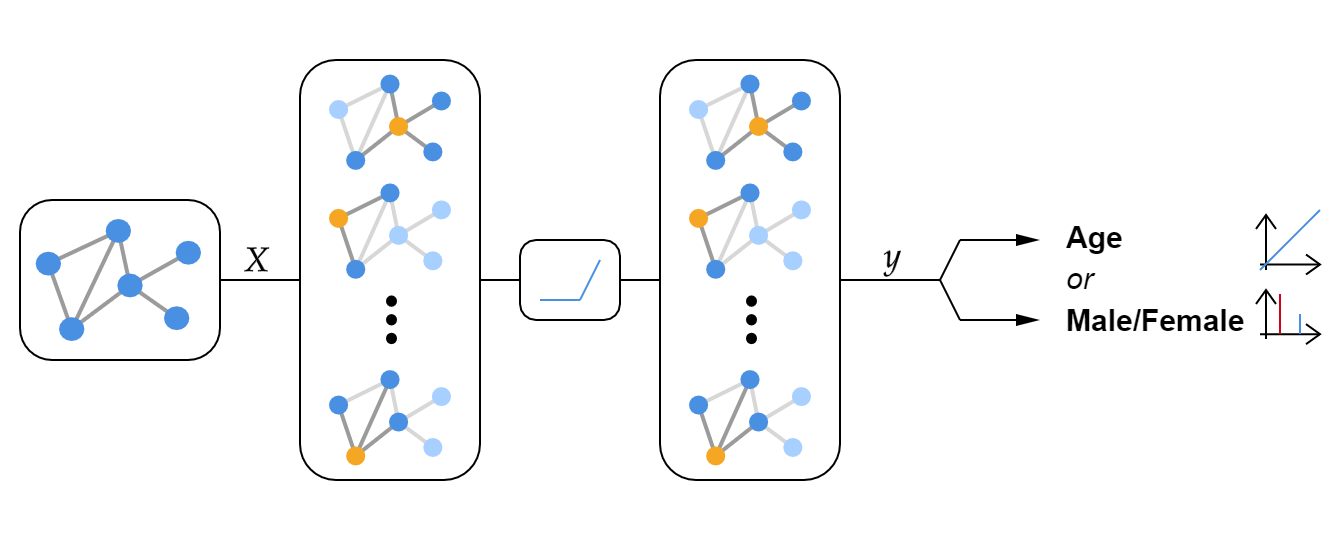
\includegraphics[width=0.9\textwidth]{chapters/images_methods/gcn.png}
    \caption{TEMP}
    \label{fig:gcn_base}
\end{figure}

An illustration of this model can be seen in figure \ref{fig:gcn_base}. And lastly to what so far been glosed over; the input features to the model. For this model the input feature matrix $X$ is chosen to be the identity matrix $I$. This is at all possible because the small size of the graphs since the number of weights for the first GCN layer scales with the number of nodes, this is not the case otherwise.

%\subsection{gcn dummy}
%The next model that will be investigated is refereed to GCNDummy which is very similar to GCNBase. They both have three GCN layer followed by a dense layer. The only difference is that while GCNBase has the identity matrix as input features while GCNDumy has a column of ones as input features. This model will thus be equivalent to placing the value of one at each node and then propagate all the ones with message and thus only evaluate how well connected every node is with its immediate surroundings.  
%\subsection{gcn features}
%\subsection{Node shuffling}
%Node shuffling

\section{Node classification -- population graphs}
In the next part of the thesis we investigate how well models involving population graphs perform. In this case since each node in the population graph is a subject the models need to do node predictions instead of graph predictions. 

\subsection{Forming population graphs}

As discussed in section \ref{sec:ml_on_graphs}, population graphs are a special type of graph in which each node corresponds to a subject, with the edges of the graph connecting the subjects being calculated using a similarity measure. The design of this similarity measure is an important decision, which should be done with the given application in mind. In our case, we want subjects that have similar fMRI data to be connected with edges that have a large weight, with the idea that our models will be able to draw upon this information on similarity to yield a better inference. Given two subjects and their adjacency matrices $A_1$ and $A_2$, we define the similarity measure $\sigma\left(A_1, A_2, l\right)$ as

\begin{equation}
    \sigma\left(A_1, A_2, l\right) = \exp{\left(- \frac{||A_1 - A_2||_F}{l ||A_1||_F ||A_2||_F} \right)},
    \label{eq:similarity_measure}
\end{equation}
where $||A_1 - A_2 ||_F$ is the matrix Frobenius norm of the difference between $A_1$ and $A_2$. The Frobenius norm is defined as $||A||_F = \left( \sum_i \sum_j |A_{ij}|^2 \right)^{1/2}$. The norm of the difference is weighted with a hyperparameter $l$ and the norms of $A_1$ and $A_2$, and then fed into an exponential kernel. The exponential kernel ensures that larger differences between $A_1$ and $A_2$ yields smaller similarity scores $\sigma\left(A_1, A_2, l\right)$, and also that  $\sigma\left(A_1, A_2, l\right) \in \left[0, 1\right]$. As desired, subjects that have similar fMRI data, and thus a smaller difference between their adjacency matrices, will with equation \eqref{eq:similarity_measure} obtain a larger similarity score and vice versa. 

Note that our similarity measure in equation \eqref{eq:similarity_measure} only draws use of the fMRI data for each subject. One could imagine a similarity measure that uses other types of data that is related to our tasks of predicting age/sex, such as eventual brain-health related diagnosis \cite{stankeviciute}. We decided to limit ourselves to only using fMRI data for two reasons; partly because using other data sources requires extensive domain knowledge, and partly because we are specifically interest in the predictive power of fMRI data, without introducing other confounding variables. 


% \subsection{Network architectures}
\subsection{Baseline model}
As a baseline model for doing predictions on a population graph a model similar to GCNBase is used. The model takes in the population graph propagates it through five GCN layers. 
Afterwards instead of feeding all activation's to a dense layer all activation's for every feature in all layers for a specific node is feed to a dense layer. This dense layer gives a prediction for the specific nodes. This is then repeated for all the nodes with the same dense layers which then gives a prediction for all nodes in the graph, see figure \ref{fig:poptoy} for an illustration of the model. 

\begin{figure}[H]
    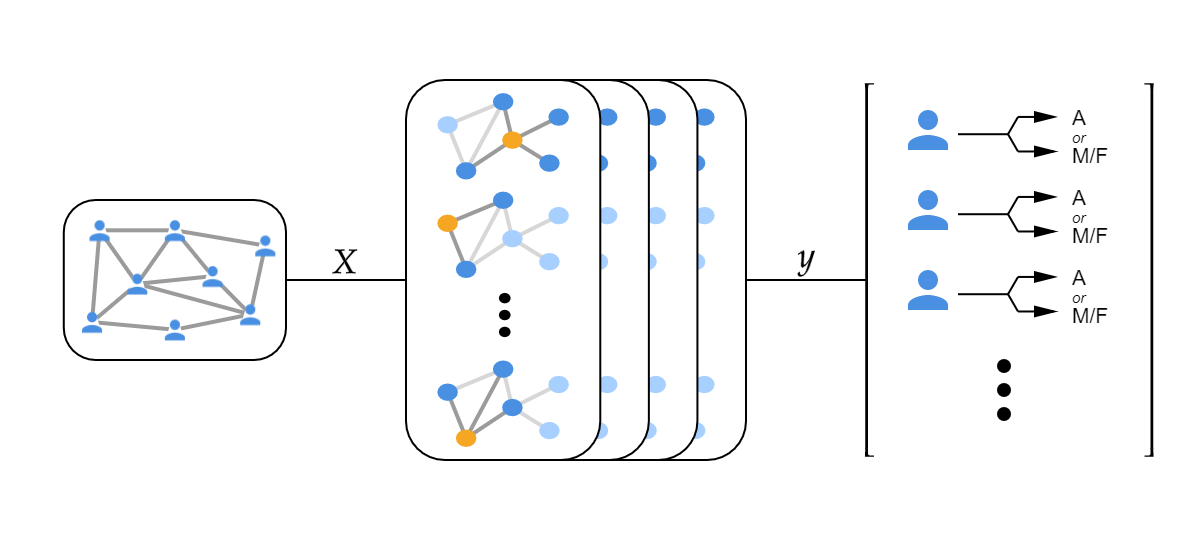
\includegraphics[width=0.9\textwidth]{chapters/images_methods/poptoy.png}
    \caption{TEMP}
    \label{fig:poptoy}
\end{figure}


%Afterwards instead of concatenating all activation's for all nodes and feed them to a dense layers we concatenate all activations for every node, see figure \ref{} for illustration. Then a kind of convolution is used where all the activation's for a specific node is feed to a dense layer and a prediction made.
Since all subjects in the data set is incorporated in the population graphs the split into validation and training set must be handled. The solution is given by defining a set of subject that will be the training set and another that will be the validation set, and the population graph thus have one set of nodes considered to be training nodes and one set to be validation nodes. The model was then constructed so it could either do predictions for only the nodes in the training set or validation set. Then the training could be performed while we only did the prediction and training on the training set and vice versa when evaluating.

%\subsection{POPToy w. dummy}
%\subsection{POPToy w. features (fmri)}
\subsection{POPEncoder}
As a means to incorporate more information about each subject in the population graph a model refereed to as POPEncoder is investigated. In this model features are introduced to the population graph. The features are based on adjacency matrix of each individual subject, but to compress the dimensionallity of the feature space we want to encode these matrices into a lower dimensional space. An heuristic explanation of how this would help is that the encoder can make an initial prediction of the age or sex of each individual subject. And then by propagating this information through the population graph the information of similarities to other subjects in the dataset possibly can improve on the predictions. Their exist many ways of performing the encoding, for example it can be done as a preprocessing step by performing predictions with one of our previous models which will get it to one or two features. In POPEncoder the encoder is however viewed as a trainable part of the model which allows possibly more advantageous embeddings then an initial prediction. 

%POPEncoder can be seen as a combination of a model for graph predictions with a model for node predictions as been hinted before one hope is that the encoder should be able to make an initial prediction and by propagating that prediction through the population graph the model could be able to utilize similarities and structure in the hole population.

\section{Batches of population graphs}
Since a population graph is a graph where each node represent a single subject and the number of edges of the graph grows with the number of nodes squared the adjacency matrix for the population graph quickly becomes very larger. This is a big problem since doing prediction and training with such a large matrix becomes very time consuming and also memory consumption can become problematic. To resolve this problem and thus in a feasible way be able to train on population graphs that includes all the data a batching method was developed. 

\begin{figure}[H]
    \centering
    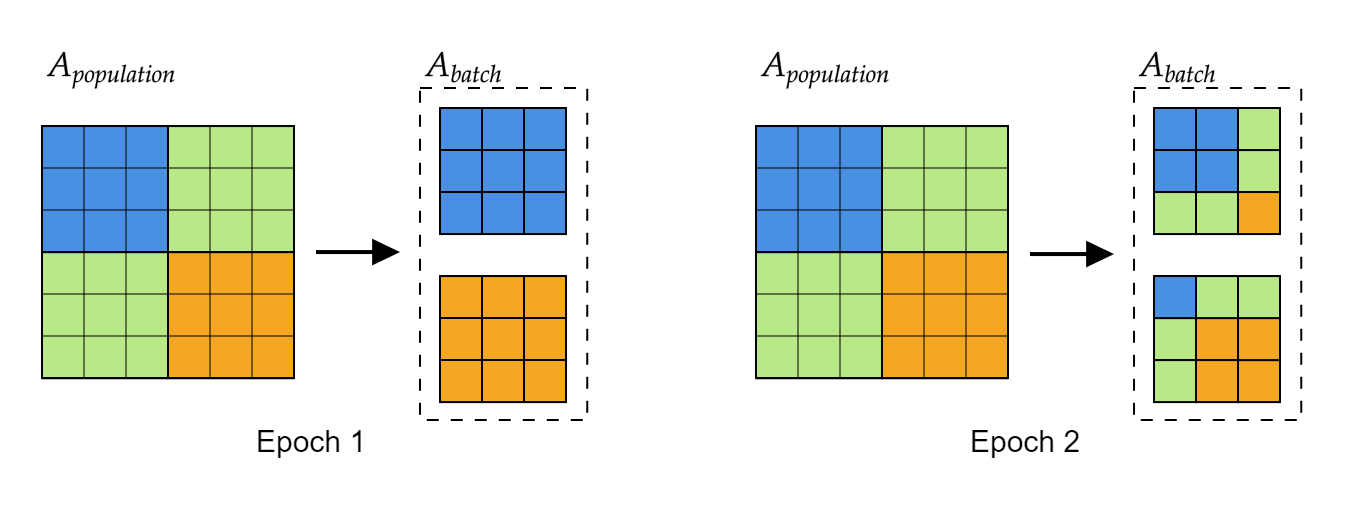
\includegraphics[width=0.9\textwidth]{chapters/images_methods/batches.png}
    \caption{TEMP}
    \label{fig:batches}
\end{figure}

The batching method was based on dividing the population graph into several smaller population graphs. For an illustration on how this can be done see figure \ref{fig:batches}. For example a population graph with 10 000 subjects would have an adjacency matrix with 1e$^8$ entries which takes about 800 MB to store in memory. However if the same population graph is divided into 100 smaller population graphs with 100 subjects in each graph the total number of entries needed to be stored would be 1e$^6$ corresponding to about 8 Mb of memory. And if the size of the smaller population graphs remains constant the memory and computation times grows linearly when adding more subjects to the data set instead of quadratic.

As seen in figure \ref{fig:batches} many of the connection between subjects is not utilized if the population graph is divided into several smaller graphs. To solve this the way the subjects are divided into smaller graphs is changed between epochs as seen in figure \ref{fig:batches}. By always changing which people are combined in the graphs all connections will potentially be used after enough epochs. The advantage of of always changing the subjects that are included in the graphs is that the model can't over fit against a specific graphs structure. The models are thus forced to learn very general patterns to classify all the subjects in the graphs. 




\section{Analysis}
Since the goal of the thesis is not only to construct models to achieve good performance, but also to determine interesting biomarkers and understand the changes in the brain between both young/old and male/female brains, analyse the model is a important part of the work. The methods for doing this can in crude way be divided into methods that open the black box and methods that do not. The black box referees to the the model since they are generally hard to understand, and opening them up refers to understanding the models by directly investigating them for example by studying weights, activation's and gradients. Below a couple methods we used out of many available methods for analysing models will be presented. 


\subsection{Model analysis/evaluation}
\subsection{Node masking}
A first very simple method to investigate what information is important  for doing predictions is a masking method, which is black box method. This particular masking method is a self-composed method based on simply removing a specific node or connection for every subject in the dataset and then retrain a new model. By masking every connection and node one at a time and then compare each models performance to a baseline where all information is utilized information of how important each node and connection is for the prediction can be extracted. This method is potentially also viable when not retraining the models, i.e. doing prediction on masked data with a model trained on unmasked data. This could however be problematic since the question of how to mask the nodes so worse performance means less importance. This problem arises since the absence of a connection not is the same as an uninformative connection. The model can for example assume some connection which is fairly constant across the dataset, removing this node may leed to significant worse performance even if it's not related to age or sex.

\subsection{Node masking: Zorro}
Another masking method for analysing neural network models with graphs as input is the Zorro algorithm \cite{}. This algorithm is by the writers introduced for analysing models performing semi-supervised node classification. This means that the dataset consists of one big graph with one adjacency matrix and one feature matrix. Since we are doing graphs classification where each subject has a unique adjacency matrix some alterations must be done to the algorithm. First we, in a big picture, describe how the Zorro algorithm works and then what alterations have been made by us.

To describe the Zorro algorithm we introduce a model $\Phi_n(X,A)$ which takes as input an adjacency matrix and a feature matrix and gives a prediction for each node $n$. The general idea is to replace the feature matrix $X$ by noise and then reintroduce nodes and feature which makes the model prediction similar to the original. The way the noise is introduced is by 
\begin{equation*}
    Y_s = X \odot S + Z \odot (1- S), \quad Z \sim \mathcal{N}, 
\end{equation*}
where $S = \{V, F\}$ is refereed to as a explanation where the nodes $V$ and features $F$ is unmasked. The noise $\mathcal{N}$ is proposed by the authors of \cite{} to be set to the distribution of the dataset. The prediction of the model $\Phi$ on the masked data is then $\Phi_n(Y_s, A)$. To evaluate an explanation $S$ i.e. if a node and feature is important for the prediction of a specific node the fidelity of the explanation is calculated by
\begin{equation*}
    \mathcal{F}(S) = \mathbb{E}_{Y_s|Z\sim\mathcal{N}}[1_{\Phi_n(X,A) = \Phi_n(Y_s,A)}].
\end{equation*}
The fidelity of an explanation is a measure of how likely it is for a model with a masked dataset to give the same prediction as model with the original dataset. The algorithm then consists by iterative add the node or feature that increases the fidelity the most until the fidelity of an explanation is higher then $\tau$, which can be chosen.

Now to what modification that have been made to the algorithm to suit our models. First of all both GCNBase and the baseline model for individual graph prediction are completely featureless approaches that only takes an adjacency matrix as input and give one prediction per graph. Therefore it is note possible to mask the feature matrix and it must be done on the adjacency matrix. The unmasking can be done in two ways either on a connection level where entries in the adjacency matrix is unmasked or on a nodal level were hole rows and columns in matrix are unmasked. Since we primarily are interested in which nodes are important we decided on the latter, which also has computationally benefits. An explanation $S = \{V\}$, thus now only contains a set of nodes to be unmasked. The mask is now given by 
\begin{equation*}
    B_S = A \odot S + Z \odot (1- S), \quad Z \sim \mathcal{N},
\end{equation*}
and the model predictions as $\Phi(A)$ and $\Phi(B_S)$. The noise is drawn from a Gaussian distribution with mean and standard deviation given by the entries of $A$ over the dataset. The fidelity are calculated in the same way and an explanation for a individual subject is still accepted if the fidelity of the explanation is higher then $\tau$. Lastly since the algorithm gives which nodes are important for the prediction of a individual subject the procedure is repeated for several subjects and the final score indicating how important a node is is given by the number of time the node was included in the explanations. 


%This algorithm is by the writers introduced which nodes and features are important when the model are doing node predictions. Since the models we analys is graphs calssifications models some alterations are needed. Furthermore the algorithm is designed for datasets with a constant node 

%ZORRO is based on replacing all the entries of the feature matrix by random noise. By then reintroduce features and nodes by demasking them and selecting nodes and features that gives the most similar performance as the original performance 

\subsection{Salience mapping, GRAD-CAM}
Another method not utilizing different kinds of masking algorithms are the GRAD-CAM method which is a method for opening up the black box. The basic principle of the GRAD-CAM algorithm is to study activations of different graph-nodes in the model when predictions are made. By identifying the nodes where the activations impact the predictions the most important graphs-nodes can be identified. 

The GRAD-CAM algorithm was initially made for convolutional neural network where important pixels in a image was identified \cite{} but was generalized to GCNs in \cite{}. The algorithm calculates the importance score for node $n$ at the GCN layer $l$, for class $c$ by 
\begin{equation*}
    L_c[l,n] =  \text{RELU}(\sum_k \alpha^{l, c}_k F_{K,n}^l). 
\end{equation*}
Here $F_{K,n}^l$ is the activations of the $k$-th feature of the $l$-th GCN layer at node $n$ and $\alpha^{l, c}_k$ is a set of class specific weights for layers $l$ given by 
\begin{equation*}
    \alpha^{l, c}_k = \frac{1}{N}\sum_{i = 1}^N \frac{\partial y^c}{\partial F^l_{k,n}}.
\end{equation*}

This algorithm depends on the architecture of the model having a GAP layer between the last GCN layer and the fully connected output layer. A GAP layers is average global pooling layer which averages all the features of the last layer over the nodes before passing them to the dens layer. This is a big problem since GCNBase has primarily two significant differences. The first one being that GCNBase does not utilize any GAP layer before the output layer and thus has a specific weight for all nodes and features not only one weight per feature. The second problem is that GCNBase in addition to the activations of the last GCN layer also utilizes the activations of all previous GCN-layers. The solution to these problem is to do some slight alterations to the GRAD-CAM algorithm in the form of 
\begin{equation*}
    L_c[l,n] =  \text{RELU}(\sum_k \alpha^{l, c}_{k,n} F_{K,n}^l)
\end{equation*}
and
\begin{equation*}
    \alpha^{l, c}_k = \frac{\partial y^c}{\partial F^l_{k,n}}.
\end{equation*}
